%!TEX root = ../main.tex

\chapter{Schematic Editor}

The first step in every project is schematic capture.
If this term is unfamiliar, we are referring to the process of laying out the components and connections between them in logical, well-defined fashion.
You may have only the barest idea of the circuit aspects or you may have the major aspects already sketched on paper;
whatever your situation, transferring the schematic into KiCad begins with the Schematic Editor.

Before we dive into the simplistic aspects of the schematic editor, it will pay us dividends later to properly understand how the schematic editor views more complex schematics.
This will allow you to structure the schematic in your mind more closely to how Schematic Editor expects.

\section{Hierarchical Schematics Explained}

The basic, underlying paradigm of the Schematic Editor is the idea of \textit{hierarchical schematics}.
If the overall schematic represents the full circuit that will exist on the circuit board at the end of production, then the hierarchy provides a logical grouping of similar component sets.
This allows you to reuse common subsets throughout your design.
The hierarchy also explicitly structures your schematics as a top-down tree.
\begin{figure}
	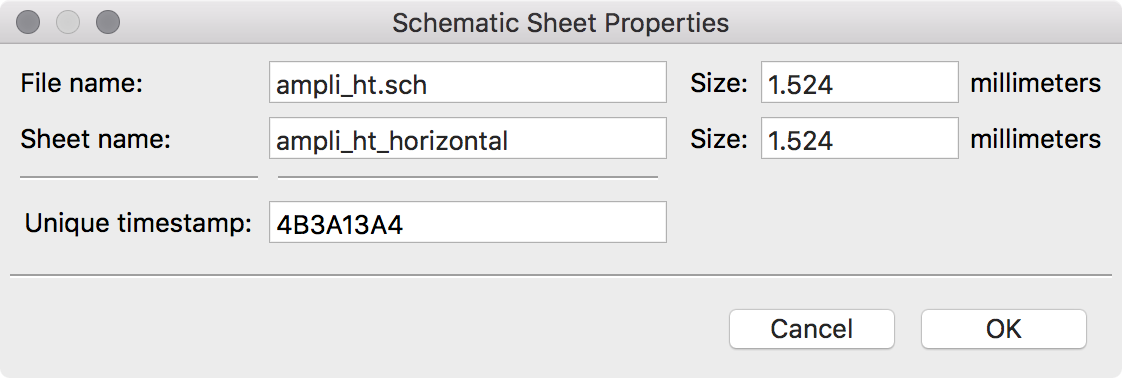
\includegraphics{chapter5/subsheet.png}
	\caption[Sub-Sheets]{The subsheet dialog specifies the file name, sheet name and a unique timestamp.}
\end{figure}

At the root of the tree, is the first schematic sheet you open, usually with the same name as your project and the extension `\textbf{.sch}'.
Off of this root, you can create \textit{sub-sheets} that are placed in the root sheet.
The sub-sheet has both a ``File name'' and a ``Sheet name''.
The File name is the name of the sub-sheet on the underlying filesystem.
This is the name you will see if you open your project folder outside of KiCad.
The Sheet name is the internal reference of the specific \textit{instance} of the sub-sheet in KiCad.

One of the primary benefits of this setup is the ability to organize the relationship between subsheets.
It can also allow you to create and re-use common elements between projects.
This will be useful when we begin discussing design reuse in section \ref{sec:reuse}.


\section{Understanding the Schematic Editor}
\begin{figure*}
    \begin{tikzpicture}[baseline]
    \begin{scope}
        \node[anchor=south west,inner sep=0] (image) at (0,0) 
        	{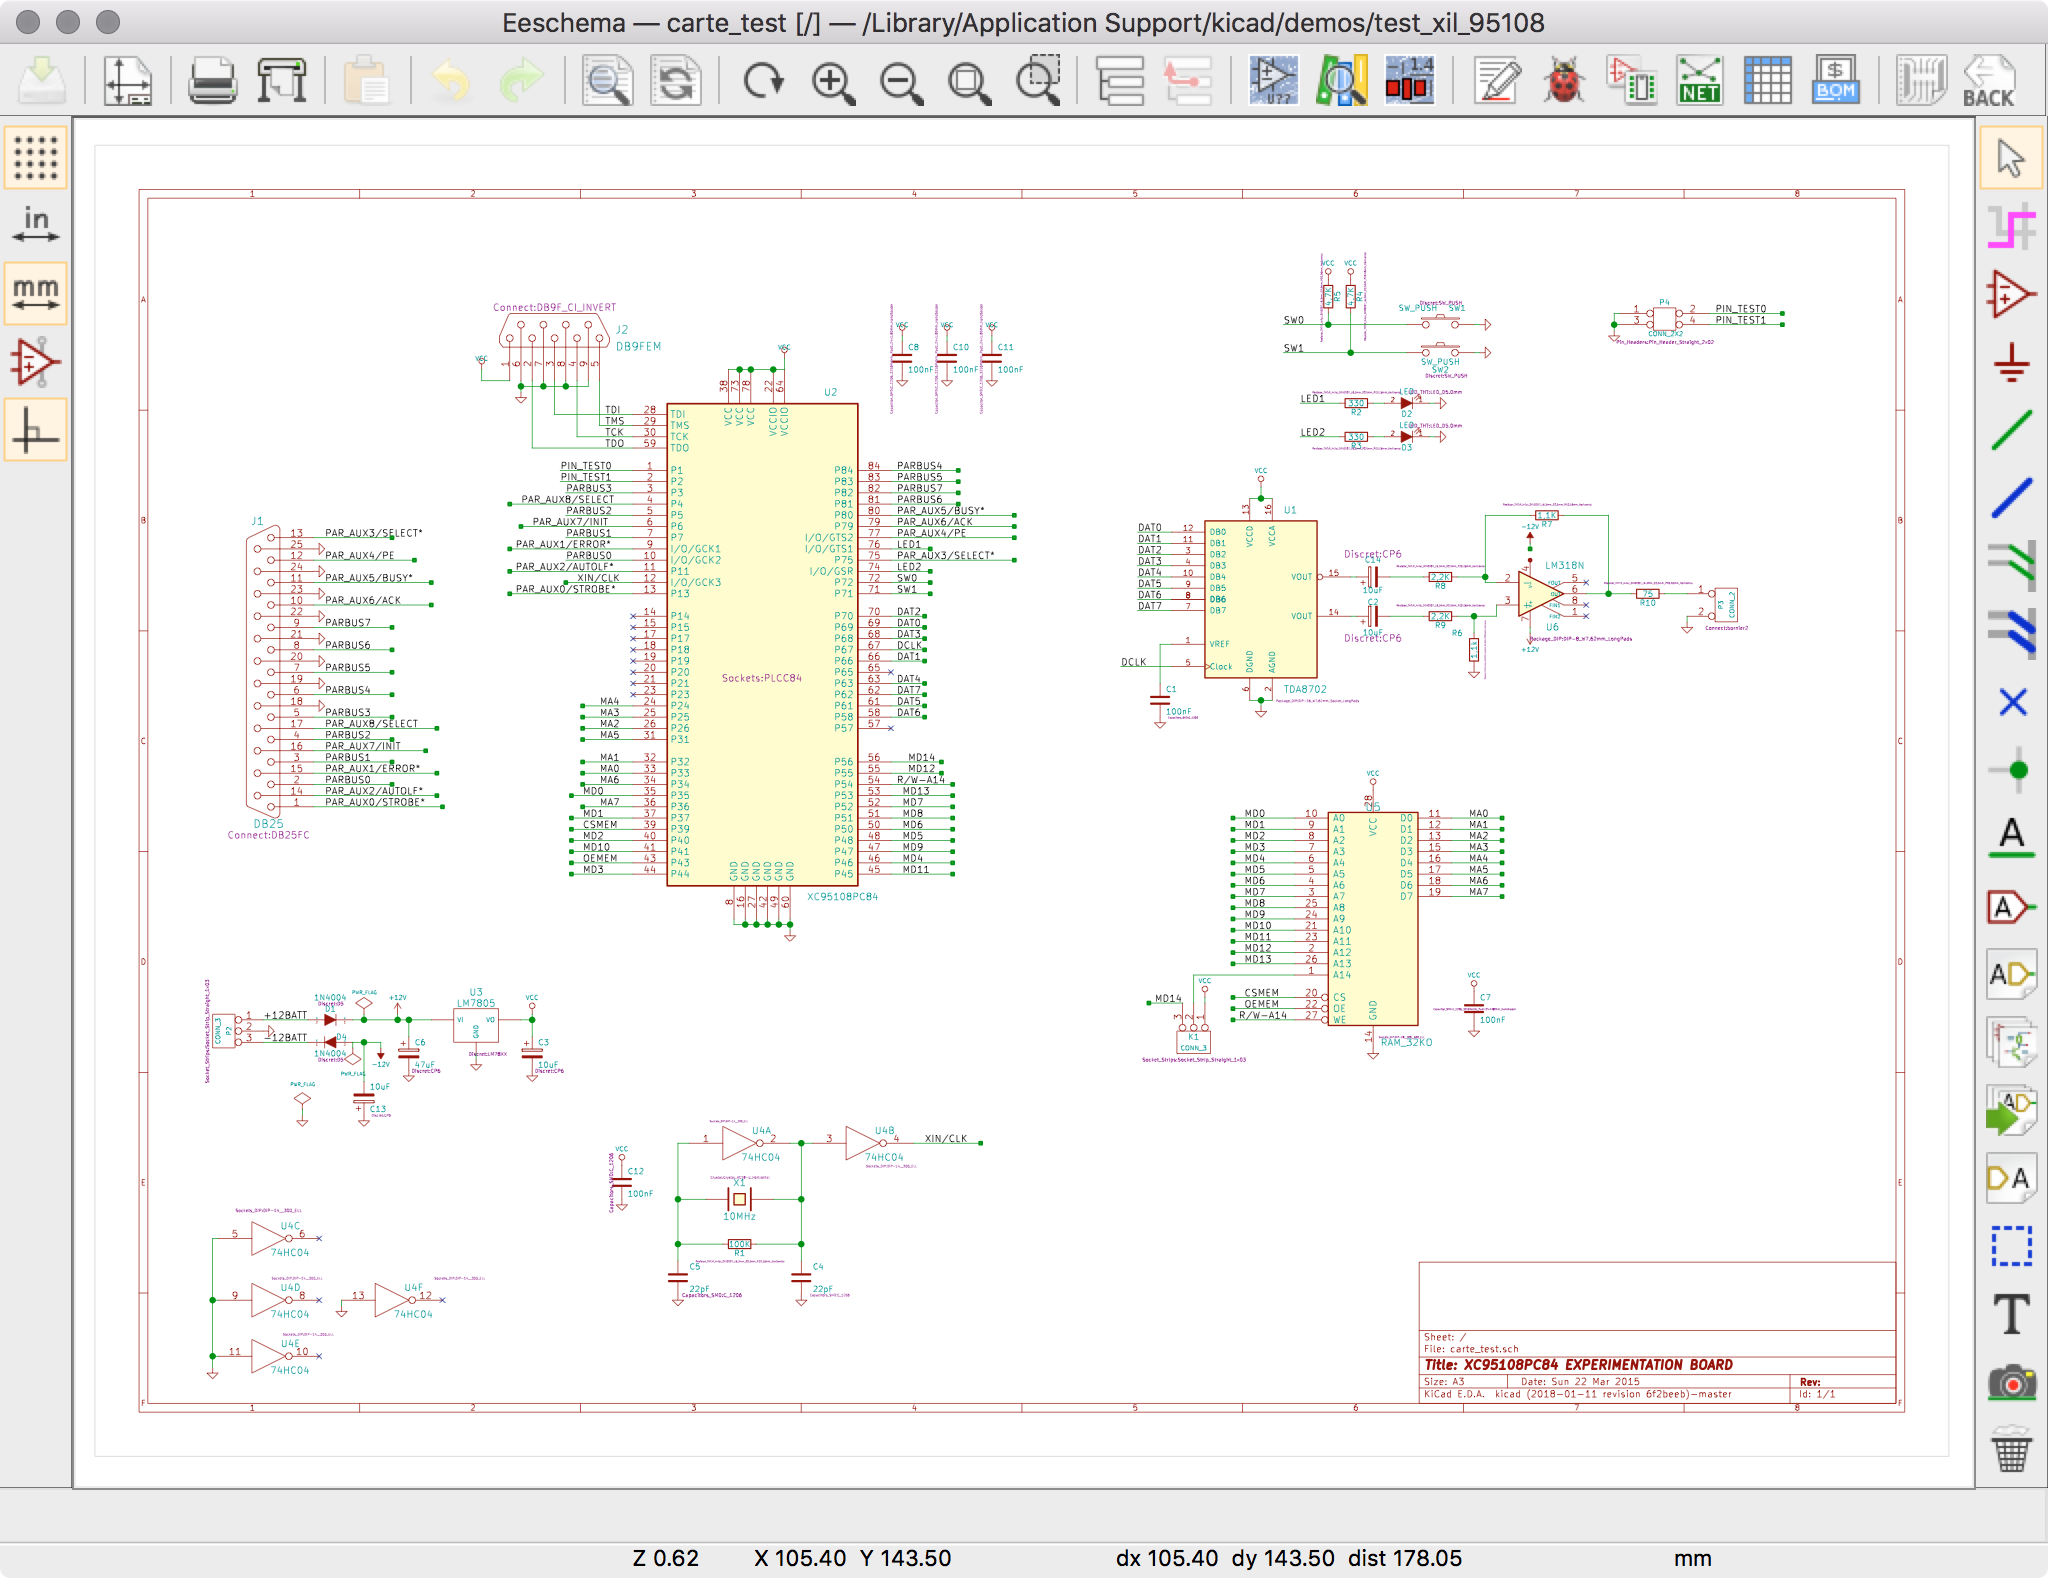
\includegraphics[width=4.5in]{chapter5/eeschema-main.png}};
        \begin{scope}[x={(image.south east)},y={(image.north west)}]
            \node [anchor=south] (file) at (0.08,1.0) {\Large File\strut };
            \node [anchor=south] (edit) at (0.2575,1.0) {\Large Edit\strut };
            \node [anchor=south] (view) at (0.438,1.0) {\Large View\strut };
            \node [anchor=south] (app) at (0.763,1.0) {\Large Applications\strut };
            \node [anchor=south, rotate=-90] (tools) at (1.0,0.5) {\Large Schematic Tools};
            \node [anchor=north, rotate=-90] (options) at (0.0,0.5) {\Large Display Options};
            
%            \draw[help lines,xstep=.05,ystep=.05] (0,0) grid (1,1);
            \draw[red,thick,rounded corners] (0.0,0.923) rectangle (0.155,0.97);
            \draw[red,thick,rounded corners] (0.162,0.923) rectangle (0.35,0.97);
            \draw[red,thick,rounded corners] (0.357,0.923) rectangle (0.525,0.97);
            \draw[red,thick,rounded corners] (0.60,0.923) rectangle (1.0,0.97);
            \draw[black!80,thick, dashed, rounded corners] (0.961,0.92) rectangle (1.0,0.05);
            \draw[black!80,thick, dashed, rounded corners] (0.0,0.92) rectangle (0.039,0.7);
            \draw [-latex, thick, red] (file.base) -- ++(0,-0.05);
            \draw [-latex, thick, red] (view.base) -- ++(0,-0.05);
            \draw [-latex, thick, red] (edit.base) -- ++(0,-0.05);
            \draw [-latex, thick, red] (app.base) -- ++(0,-0.05);
            \draw [-latex, thick, dashed, black!80] (tools.west) to[out=90, in=-20] (1.0,0.85);
            \draw [-latex, thick, dashed, black!80] (options.west) to[out=90, in=-160] (0.0,0.85);
        \end{scope}
    \end{scope}
    \end{tikzpicture}
	
	\caption[Eeschema]{The Eeschema main window.  Control buttons on the top}
\end{figure*}
\subsection{Relationship to Symbol Libraries}
\subsection{Project Settings}

\section{Adding Parts}

\section{Connections}
\subsection{Wires}
\subsection{Busses}
\subsection{Labels}
\subsection{Junctions}
\subsection{No Connects}
\subsection{Hierarchical Pins}

\section{Electrical Rules Check}

\section{Graphical Elements}

\section{Templates}

\section{Schematic Editor Examples}
\subsection{Example 1: Single Page Schematic}
\subsection{Example 2: Hierarchical Schematic}